\newcommand\gauss[2]{1/(#2*sqrt(2*pi))*exp(-((x-#1)^2)/(2*#2^2))} % Gauss func

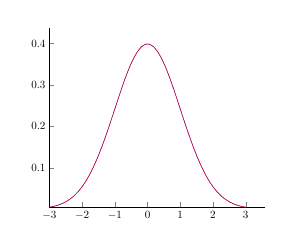
\begin{tikzpicture}[scale=.4, transform shape]

	\begin{axis}[every axis plot post/.append style={
				mark=none,domain=-3:3,samples=50}, % All plots: from -2:2, 50 samples, smooth, no marks
			axis x line*=bottom, % no box around the plot, only x and y axis
			axis y line*=left, % the * suppresses the arrow tips
		enlargelimits=upper] % extend the axes a bit to the right and top
		
		\addplot {\gauss{0}{1}};
		\addplot {\gauss{0}{1}}[scale=.5];
	\end{axis}
	
\end{tikzpicture}